\subsection*{Global Structures}
    \emph{``Global''} structures here refer to those that are defined via integrals over $\bfOmega$, i.e. those that are functions of $t$ only.

    Define first the general \emph{``helicity''}, $\calH[\bff](t)$, of a vector field $\bff : \bfOmega\otimes\bbR \rightarrow \bbR^{3}$: \cite{Moffatt_1969, Brown_Canfield_Pevtsov_1999}
    \begin{equation}
        \calH[\bff](t)  :=  \int_{\bfOmega}\bff\cdot(\nabla\wedge\bff)|_{t}
    \end{equation}
    Helicity can be interpreted topologically as a continuous analogue to the linking number in knot theory, a topological invariant for pairs of closed curves in $\bbR^{3}$. \cite{Berger_1999} (See Figure \ref{fig:linking numbers})

    \begin{figure}[!ht]
        \centering
        \begin{subfigure}{0.1868\textwidth}
            \centering
            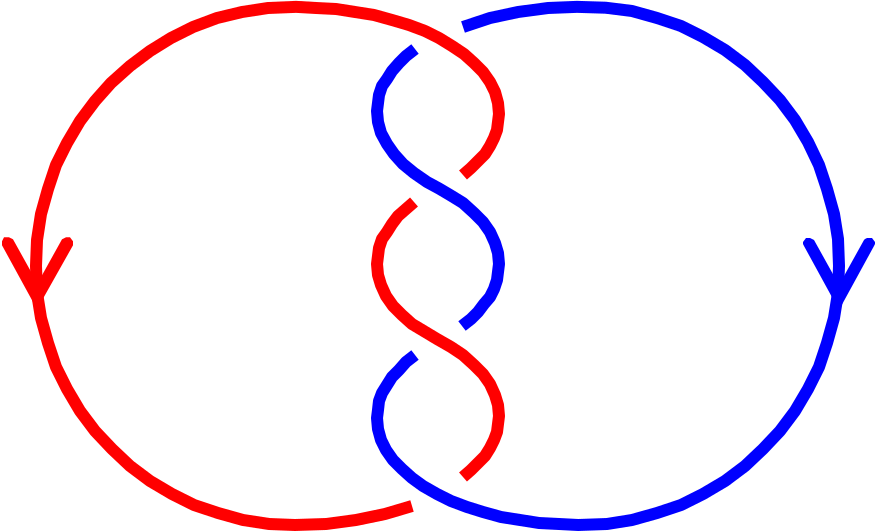
\includegraphics[width = 0.75\textwidth]{2 - fluid component/1 - structures/2 - global/images/-2.png}
            \caption{$L = -2$}
        \end{subfigure}%
        \begin{subfigure}{0.1811\textwidth}
            \centering
            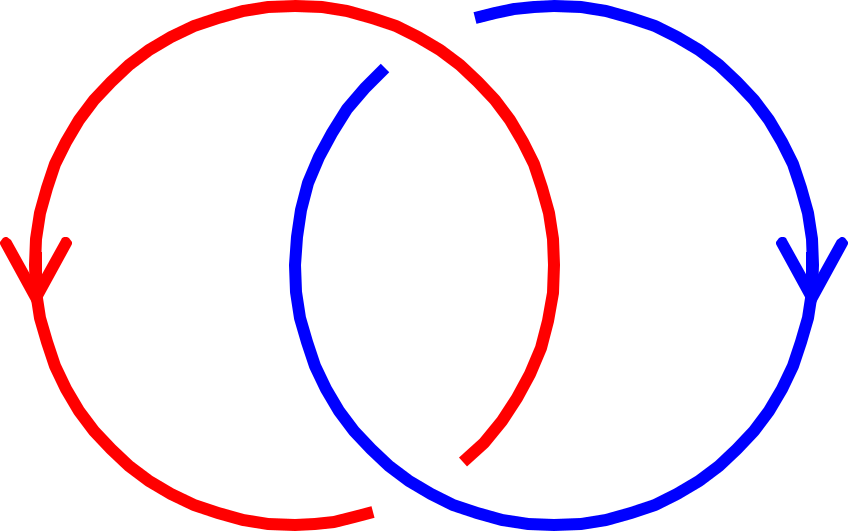
\includegraphics[width = 0.75\textwidth]{2 - fluid component/1 - structures/2 - global/images/-1.png}
            \caption{$L = -1$}
        \end{subfigure}%
        \begin{subfigure}{0.2634\textwidth}
            \centering
            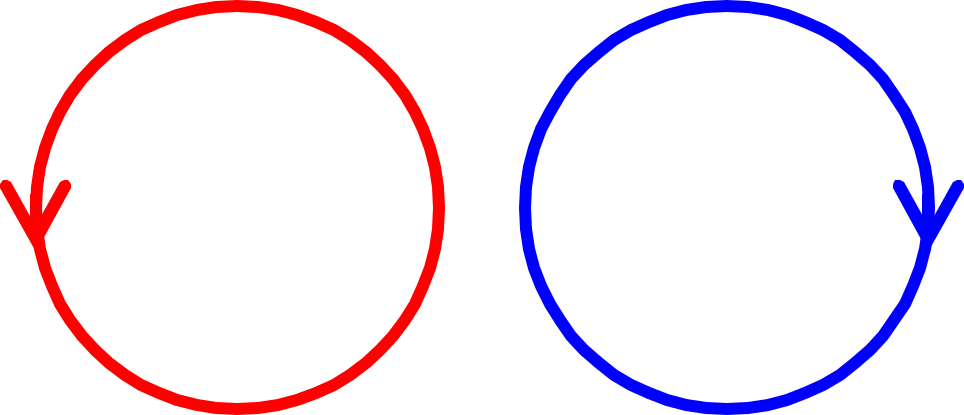
\includegraphics[width = 0.75\textwidth]{2 - fluid component/1 - structures/2 - global/images/0.png}
            \caption{$L = 0$}
        \end{subfigure}%
        \begin{subfigure}{0.1815\textwidth}
            \centering
            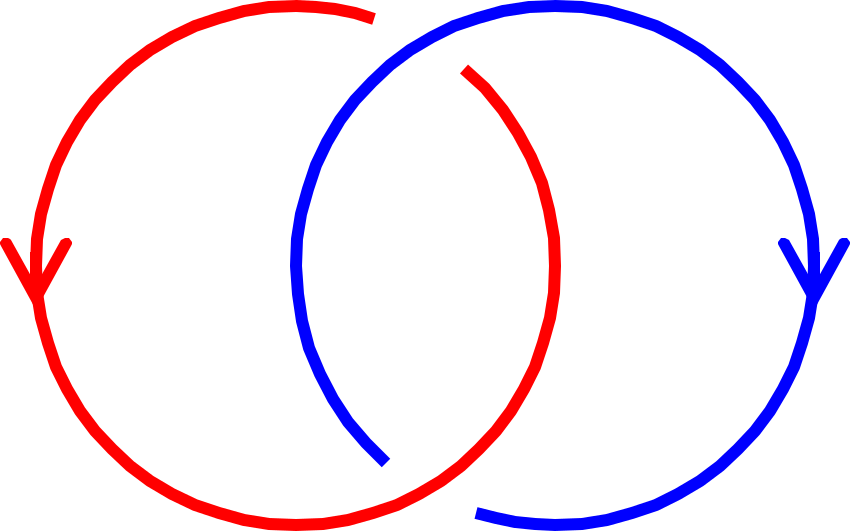
\includegraphics[width = 0.75\textwidth]{2 - fluid component/1 - structures/2 - global/images/1.png}
            \caption{$L = 1$}
        \end{subfigure}%
        \begin{subfigure}{0.1872\textwidth}
            \centering
            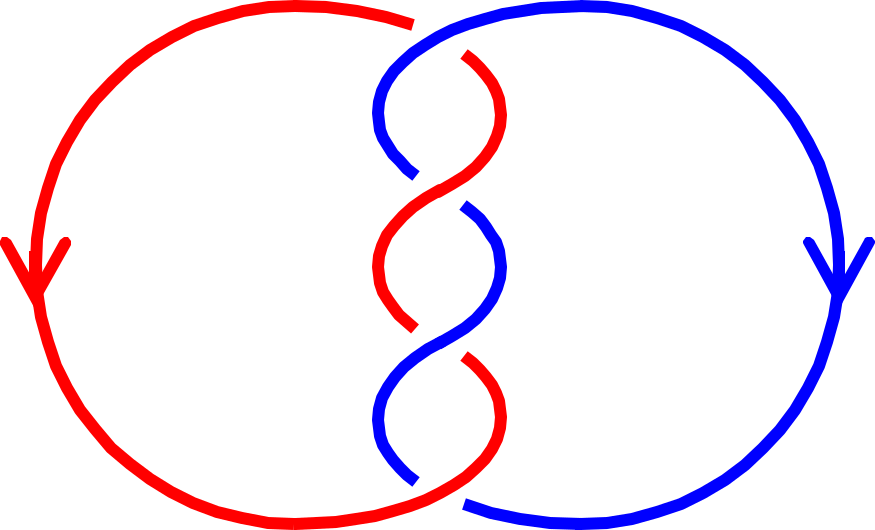
\includegraphics[width = 0.75\textwidth]{2 - fluid component/1 - structures/2 - global/images/2.png}
            \caption{$L = 2$}
        \end{subfigure}
        \caption{Examples of pairs of closed loops in $\bbR^{3}$ with linking numbers $L  \in  \{-2, -1, 0, 1, 2\}$. Vector fields with correspondingly varying helicities exhibit similar twisting structures.}
        \label{fig:linking numbers}
    \end{figure}
    
    \begin{remark}
        We call this $\bfA$ \emph{a}, not \emph{the}, magnetic potential since a continuum of such magnetic potentials can exist, up to the addition of a vector field in the kernel of $\rmdiv$, i.e. a potential gradient.
        
        It is irrelevant however here which potential $\bfA$ is chosen, as the conservation/dissipation results still hold.
    \end{remark}

    Assume henceforth the homogeneous boundary conditions (BCs) on $\bfGamma$:
    \begin{align}\label{eqn:canonical boundary conditions}
        \bfzero  =  \bfu\cdot\bfn,   &&
        \bfzero  =  \bfB\cdot\bfn,   &&
        \bfzero  =  \bfE\wedge\bfn.
    \end{align}

    Denote a magnetic potential, $\bfA$, defined such that $\bfB  =  \nabla\wedge\bfA$ with BCs $\bfzero  =  \bfA\wedge\bfn|_{\bfGamma}$. By the exactness of the $\Lambda_{0}^{\bullet}(\bfOmega)$ Hilbert complex on contractible $\bfOmega$ (See Appendix \ref{cha:Hilbert complexes}) such a potential necessarily exists, since
    \begin{equation}
        \bfB  \in  \ker[\rmdiv; \bfH_{0}(\rmdiv)]  =  \im[\bfcurl; \bfH_{0}(\bfcurl)].
    \end{equation}

    \begin{remark}
        Various other BCs are considered in the literature ($\bfzero = \bfu\wedge\bfn$, $\bfzero = \bfB\wedge\bfn$, etc.) however I'm choosing to consider these ones for now, since they are crucial for giving conservative/dissipative properties and the global quantities that we are to consider.
    \end{remark}

    In the incompressible case, \cite{Laakmann_Hu_Farrell_2022} considers the conservation of the following 3 quantities in the incompressible system:\footnote{Note, the hybrid helicity, $\rmH_{\rmH}$, is \emph{not} (necessarily) the helicity of a vector field, except in the case of $a = b = \beta\rmRH/2 (= 1/\rmCy\!_{+})$, where
    \begin{equation}
        \rmH_{\rmH} = \calH\left[\bfA + \frac{2}{\beta\rmRH}\bfu\right].
    \end{equation}
    It is referred to here as the hybrid \emph{helicity} here only by convention.}
    \begin{center}\begin{tabular}{ c | r : l }
        Properties  &  Symbol  &  Definition  \\
        \hline\hline
        Energy  &  $\rmE$  &  $\frac{1}{2}\|\bfu\|_{\bfOmega}^{2} + \frac{1}{\beta}\|\bfB\|_{\bfOmega}^{2}$  \\
        \hdashline
        Magnetic helicity \cite{Blackman_2015}  &  $\rmH_{\rmM}$  &  $\calH[\bfA]$  \\
        Hybrid helicity \cite{Subramanian_Brandenburg_2006}  &  $\rmH_{\rmH}$  &  $\langle(\bfA + a\bfu), (\bfB + b\bfomega)\rangle_{\bfOmega}$
    \end{tabular}\end{center}
    where $a$, $b$ satisfy the relation
    \begin{equation}
        \frac{1}{a} + \frac{1}{b}  =  \frac{4}{\beta\rmRH}  (=  2\rmCy_{+}),
    \end{equation}
    and $\bfomega$ is the vorticity $\bfomega  :=  \nabla\wedge\bfu$.
    
    For the \emph{compressible} case, one can introduce the total mass, $\rmM$, as a conserved quantity, and redefine the energy, $\rmE$, to incorporate the internal energy and variable density. The magnetic helicity, $\rmH_{\rmM}$, remains unchanged, while to the authors' knowledge the hybrid helicity, $\rmH_{\rmH}$, has no direct analogue in the compressible case:
    \begin{center}\begin{tabular}{ c | r : l }
        Properties  &  Symbol  &  Definition  \\
        \hline\hline
        Mass  &  $\rmM$  &  $\int_{\bfOmega}\rho$  \\
        Energy  &  $\rmE$  &  $\int_{\bfOmega}\left[\frac{1}{2}\rho\|\bfu\|^{2} + \rho\theta\right] + \frac{1}{\beta}\|\bfB\|_{\bfOmega}^{2}$  \\
        \hdashline
        Magnetic helicity \cite{Blackman_2015}  &  $\rmH_{\rmM}$  &  $\calH[\bfA]$
    \end{tabular}\end{center}
    These are the global structures considered by Gawlik and Gay--Balmaz in the barotropic case in \cite{Gawlik_Gay--Balmaz_2021}.

    These quantities have the derivatives:
    \begin{align}
        \frac{\rmd}{\rmd t}\rmM         &=  0  \\
        \frac{\rmd}{\rmd t}\rmE         &=  \oint_{\bfGamma}\left[\frac{1}{\rmRef}\rho\bftau\cdot\sym[\bfu\otimes\bfn] + \frac{1}{\rmPe}\rho\nabla\theta\cdot\bfn\right]  \\
        \frac{\rmd}{\rmd t}\rmH_{\rmM}  &=  - \frac{2}{\rmRem}\calH[\bfB]
    \end{align}
    Notably:
    \begin{itemize}
        \item  If both:
        \begin{itemize}
            \item  One of the ideal kinetic limit $\rmRef  \rightarrow  \infty$, the stress-free BC $\bftau\cdot\bfn  =  \bfzero|_{\bfGamma}$, or the no-slip BC $\bfu\wedge\bfn  =  \bfzero|_{\bfGamma}$, holds.
            \item  Either the ideal thermal limit, $\rmPe  \rightarrow  \infty$, or the thermal insulation BC $\nabla\theta\cdot\bfn  =  0|_{\bfGamma}$, holds.
        \end{itemize}
        then
        \begin{equation}
            \frac{\rmd}{\rmd t}\rmE  =  0.
        \end{equation}

        \item  In the ideal magnetic limit, $\rmRem  \rightarrow  \infty$,
        \begin{equation}
            \frac{\rmd}{\rmd t}\rmH_{\rmM}  =  0.
        \end{equation}
      \end{itemize}

    \line

    \begin{lemma}[Arnold's inequality (Continuity of helicity)]\label{lem:continuity of helicity}
        For any non-empty $\bfgamma  \subseteq  \bfGamma$, there exists a Poincaré constant $C_{\bfgamma}$ such that $\forall  \bff  \in  \bfH_{\bfgamma}(\bfcurl)$ (as defined in Appendix \ref{cha:Hilbert complexes}),
        \begin{equation}
            |\calH[\bff]|  \leq  C_{\bfgamma}\|\bff\|_{\bfOmega}^{2}.
        \end{equation}
    \end{lemma}
    \begin{proof}
        The proof relies on the Cauchy--Schwarz inequality in $L^{2}$ and the (generalized) Poincaré inequality in $\bfH_{\bfgamma}(\bfcurl)$. See Theorem 1.5 of \cite{Arnold_Khesin_2008}. \BA{(Note later that this holds in complex discretizations too.)}
    \end{proof}

    The following corollary is noted also in \cite{Arnold_Khesin_2008}:

    \begin{corollary}
        Lemma \ref{lem:continuity of helicity} can be applied to the specific cases of the magnetic helicity, $\rmH_{\rmM}$, giving
        \begin{equation}
            |\rmH_{\rmM}|  \leq  C_{\bfGamma}\|\bfB\|_{\bfOmega}^{2}.
        \end{equation}
        This in turn gives the lower bound on the energy,
        \begin{equation}
            \rmE  \geq  \frac{C_{\bfGamma}}{\beta}|\rmH_{\rmM}|.
        \end{equation}
    \end{corollary}

    \BA{Would like to look at how this bound changes when one switches to a non-conforming scheme.}

    \line
